
\section{Одномерная функция распределения случайной величины}

\textbf{Автор:} Полешко Анастасия Олеговна, Б-01-006

Одномерная функция распределения непрерывной случайной величины (CDF - от англ. Cumulative Distribution Function) задает вероятность того, что случайная величина $X$ примет значение меньше или равное $x$. Функция CDF обычно обозначается как $F_X(x)$ или просто $F(x)$.

Для непрерывной случайной величины $X$ функция распределения определяется следующим образом:

$$F_{\xi} (x) = P(X \leq x) = \int_{- \infty}^{\xi} f_{X}(t)dt$$

где $f_X(x)$ - плотность распределения непрерывной случайной величины $X$.

Свойства функции распределения непрерывной случайной величины: 

1. Функция распределения неубывающая: $F(x_1) \leq F(x_2)$, если $x_1 \leq x_2$.

2. Функция распределения ограничена: $0\leq F(x) \leq 1$ для всех $x$.

3. Функция распределения непрерывна справа: $\lim_{\epsilon \to +0} F(x + \epsilon) = F(x)$ для всех $x$.

4. Функция распределения имеет предел при $x\to -\infty$: $\lim_{x\to -\infty} F(x) = 0$.

5. Функция распределения имеет предел при $x\to +\infty$: $\lim_{x\to +\infty} F(x) = 1$.

Используя функцию распределения непрерывной случайной величины можно находить вероятности попадания случайной величины в интервалы, выражать их в виде интегралов и решать задачи на нахождение квантилей и моментов случайной величины.$^{\text{\cite{ShiryaevVeroyatnost1}}}$

Мы будем изучать непрерывные процессы, а потом их дискретизировать с помощью теоремы Котельникова. $^{\text{\cite{ShamarovDRP}, Лекция №1}}$

Рассмотрим теперь случай дискретной случаной величины.
 
Пусть $(\Omega, \varkappa, \mathbb{P})$ -- вероятностная модель некоторого эксперимента с конечным числом исходов $N(\Omega)$ и алгеброй  всех подмножеств П в $\Omega$, где 

$\Omega$ -- произвольное непустое множество, элементы которого называются элементарными событиями, исходами или точками;

$\varkappa$ --  сигма-алгебра подмножеств 
$\Omega$ , называемых случайными событиями;

$\mathbb{P}$ -- вероятностная мера или вероятность, то есть сигма-аддитивная конечная мера, такая что
$\mathbb{P}(\Omega) = 1.$

$N(\Omega)$ -- мощность множества $\Omega$ для случайной величины.

Вводимое сейчас (и далее — в более общем виде) понятие случайной величины призвано определить величины, характеризующие результаты «измерений» в случайных экспериментах.

\begin{definition}\label{poleshko_def_1} Всякая числовая функция $\xi = \xi(w)$, определенная на пространстве элементарных событий $\Omega$, будет называться случайной величиной.
	\end{definition}

\begin{definition}\label{poleshko_def_2} Всякая числовая функция $\xi = \xi(w)$, определенная на конечном пространстве элементарных событий $\Omega$, будет называться простой случайной величиной.
	\end{definition}

\begin{example} В модели двукратного подбрасывания монеты с пространством исходов П = {ГГ, ГР, РГ, РР} определим случайную величину $\xi = \xi(w)$ с помощью таблицы

\begin{center}
\begin{tabular}{ | c | c | c | c | c |}
\hline
w & ГГ & ГР  & РГ & РР\\ \hline
$\xi(w)$ & 2 & 1  & 1 & 0\\ \hline
 \end{tabular}
\end {center}

Здесь $\xi(w)$ по своему смыслу есть не что иное, как число «гербов», отвечающее исходу w.
\end{example}

Другим простейшим примером случайной величины $\xi$ является характеристическая функция некоторого множества $A \in \varkappa$:

\begin{center}

$\xi = I_A(w)$, где

\begin{equation*}
I_A(w) = 
 \begin{cases}
   1 &\text{ $w\in A$}\\
   0 &\text{ $w \notin A$}
 \end{cases}
\end{equation*}

\end{center}

Когда экспериментатор имеет дело со случайными величинами, описывающими те или иные показания, то основной вопрос, который его интересует, — это вопрос о том, с какими вероятностями эта случайная величина принимает те или иные значения. С этой точки зрения интерес представляет не распределение вероятностей Р на $(\Omega, \varkappa)$, а распределение вероятностей на множестве значений случайной величины. Поскольку в рассматриваемом случае $\Omega$ состоит из конечного числа точек, то множество значений X случайной величины $\xi$ также конечно. Пусть $X = {x_1, ..., x_m}$, где (различными) числами $x_1, ..., x_m$ исчерпываются все значения $\xi$.

Обозначим $\chi$ -- совокупность всех подмножеств множества X, и пусть $B \in \chi$ . Множество В можно также интерпретировать как некоторое событие, когда пространство исходов есть X -- множество значений $\xi$.
Рассмотрим на $(X, \chi )$ вероятность $Р_{\xi}(\cdot)$, индуцируемую случайной величиной $\xi$ по формуле

$$P_{\xi} (B) = P\{ w: \xi(w) \in B\}, \ \ \ \ \ B \in \chi$$.

Ясно, что значения этих вероятностей полностью определяются вероятностями

$$P_{\xi} (x_i) = P\{ w: \xi(w) = x_i\}, \ \ \ \ \ x_i \in X$$.

Набор чисел $\{ P_{\xi} (x_1), ..., P_{\xi} (x_m)\}$ называется распределением вероятностей случайной величины $\xi$.

\begin{example} Случайная величина $\xi$, принимающая два значения 1 и О с вероятностями («успеха») р и («неуспеха») q, называется бернуллиевской. Ясно, что для нее

$$P_{\xi} (x) = p^xq^{1-x}, \ \ \ \ \ x = 0, \ 1.$$

Биномиальной (или биномиально распределенной) случайной величиной $\xi$ называется случайная величина, принимающая n + 1 значение 0, 1 , ..., n с вероятностями

$$P_{\xi} (x) = p^xq^{1-x}, \ \ \ \ \ x = 0, \ 1, \ ..., \ n.$$
\end{example}

Заметим, что в этих и во многих приводимых далее примерах мы не конкретизируем структуру основного вероятностного пространства $(\Omega, \varkappa, P)$, а интересуемся лишь значениями случайных величин и их распределениями вероятностей.

Вероятностная структура случайных величин $\xi$ полностью описывается распределением вероятностей $\{ P_{\xi}(x_i), i = 1, ..., m\}$. Вводимое ниже понятие функции распределения дает эквивалентное описание вероятностной структуры случайных величин.

\begin{definition} Пусть $x \in R^1$. Функция

$$F_{\xi}(x) = P\{ w: \xi(w) \leq x\}$$

называется функцией распределения случайной величины $\xi$. 

Ясно, что

$F_{\xi}(x) = \sum\limits_{i: x_i \leq x} P_{\xi}(x_i)$ и $P_{\xi}(x_i) = F_{\xi}(x_i) - F_{\xi}(x_i-0)$, где $F_{\xi}(x_i-0) = \lim\limits_{y \to x-0} F_{\xi}(y)$.

Если считать, что $x_1 < x_2 < ... < x_m$, и положить $F_{\xi}(x_0) = 0$, то

$$P_{\xi}(x_i) = F_{\xi}(x_i) - F_{\xi}(x_i-0), \ \ \ \ \ \ \ i = 1, ..., m$$.

\end{definition}

Приводимые далее графики дают представление о $P_{\xi}(x)$ и $F_{\xi}(x)$ для биномиальной случайной величины $\xi$.

\begin{figure}[h]
    \center 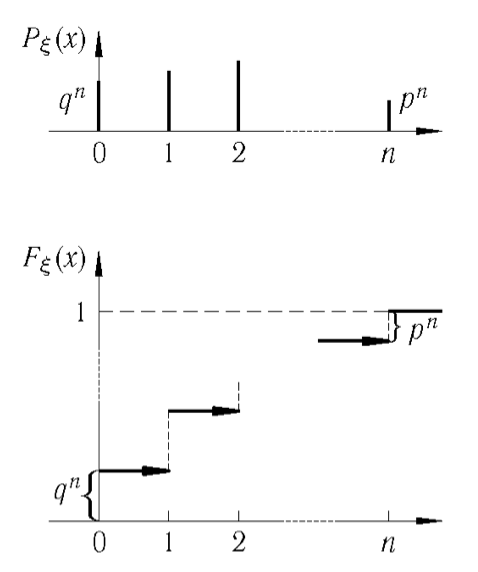
\includegraphics[scale = 0.54]{poleshko02_pic_1.png}
    \label{fig:image}
\end{figure}

Непосредственно из определения \ref{poleshko_def_2} следует, что функция распределения $F_{\xi} = F_{\xi}(x_i)$ обладает такими свойствами: 

(1)$F_{\xi}(- \infty)=0,F_{\xi}(+\infty)= 1$;

(2) $F_{\xi}(x)$ непрерывна справа $F_{\xi}(x+0) = F_{\xi}(x)$ и кусочно постоянна.$^{\text{\cite{ShiryaevVeroyatnost1}}}$


\begin{example} Приведем пример, где рассмотрим функцию распределения случайной величины, как полусумму функции распределения случайной величины, принимающей одно значение и случайной величины с гауссовской плотностью. И покажем, что эта случайная величина имеет смешанную функцию распределения, которая не сводится ни к непрерывной, ни к дискретной, ни к сингулярной.  
	\end{example}

Вспомним классификацию случайных величин:

1) дискретные. Принимают счетное или конечное число значений. Их функция распределения F(x) разрывна.

2) абсолютно непрерывные. 

$\exists p(x): F(x) = \int_{- \infty}^x p(t) dt \,$ где p(x) -- плотность распределения. Итак, $F(x) \in C$.

Пусть точка роста -- точка, где производная функции распределения не равна нулю: $x_0$: $F'(x_0) \textdoublebarslash 0$.

$X_0 = \{x_0 \in \mathds{R}|_: F'(x_0) \textdoublebarslash 0$ -- множество точек роста. Так, для абсолютно непрерывных случайных величин $mesX_0 \textdoublebarslash 0$.

3) сингулярные. Для них $F(x) \in C$, но $mesX_0 = 0$. Напомним, что для любой случайной величины: $\lim_{x\to +\infty}F(x) = 1$, $\lim_{x\to -\infty} F(x) = 0$.

Пусть $\xi_1$ имеет гауссовское распределение, $\xi_2$ -- детерминированная случайная величина. 

Плотность распределения $\xi_1$:

$$p_1(x) = \dfrac{1}{\sigma \sqrt{2\pi}} \cdot exp \left( -\dfrac{1}{2} \cdot \left(\dfrac{x - a}{\sigma}\right)^2\right);$$

А функция распределения:

$$F_1(x) = \dfrac{1}{2} \left(1 + erf\left(\dfrac{x}{\sqrt{2}}\right)\right) = \dfrac{1}{\sqrt{2\pi}} \int_{- \infty}^{x} e^{-\frac{t^2}{2}} dt, \text{где} E\xi_1 = 0, D\xi_1 = 1.$$

Для $\xi_2$:

$$p_2(x) = \delta(x-b).$$

Здесь а -- математическое ожидание $\xi_1$, b -- значение принимаемое $\xi_2$ с вероятностью 1 (пусть а \textdoublebarslash b).

Тогда функция распределения:

\begin{equation*}
F_2(x) = \uptheta = 
 \begin{cases}
   0 &\text{ $x < 0$}\\
   1 &\text{ $x \geq 0$}
 \end{cases}
\end{equation*}

Где $\uptheta$ -- функция Хевисайда.

Рассмотрим величину $\xi_3$, такую, что 

$p_3(x) = \dfrac{1}{2} \delta(x-b) + \dfrac{1}{2} \cdot \dfrac{1}{\sigma \cdot \sqrt{2\pi}} \cdot exp \left( -\dfrac{1}{2} \cdot \left(\dfrac{x - a}{\sigma}\right)^2 \right)$;

Тогда находим функцию распределения:

$$F_3(x) = \dfrac{1}{2} \uptheta + \dfrac{1}{4} \left(1 + erf\left(\dfrac{x} {\sqrt{2}}\right)\right) = \dfrac{1}{2} \uptheta + \dfrac{1}{2\sqrt{2\pi}} \int_{- \infty}^{x} e^{-\frac{t^2}{2}} dt$$

Соотвествующая плотности $p_3(x)$ функция распределения $F_3(x)$ разрывна, что доказывает невозможность $\xi_3$ быть абсолютно непрерывной или сингулярной. Более того, $\xi_3$ имеет множество значений, которое ни конечно, ни счетно, а значит $\xi_3$ не дискретная. Итак, $\xi_3$ не принадлежит ни одной из 3 категорий. 


